\section{Motivation}
\lecdate{09.01.2018}
\paragraph{Ziel}
Repräsentation der Eingabedaten erzeugen, die
\begin{itemize}
\item sowohl deren Statistik
\item als auch deren Klassenzugehörigkeit
\end{itemize}
berücksichtigt.

\paragraph{Vorgehen} Anzahl $M$ Referenzvektoren sollen eine Anzahl $P$ Datenpunkte repräsentieren/abbilden:
\begin{center}
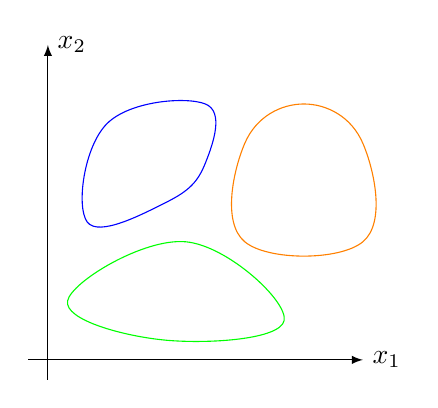
\begin{tikzpicture}[scale=.5]
\draw [-latex] (-.5,0) -- (8,0) node[right]{$x_1$};
\draw [-latex] (0,-.5) -- (0,8) node[right]{$x_2$};
\draw [blue] plot[smooth cycle, tension=.7] coordinates {(1.5,6) (1,3.5) (3,4) (4,5) (4,6.5)};
\draw [orange] plot[smooth cycle, tension=.7] coordinates {(6.5,6.5) (5,5.5) (5,3) (8,3) (8,5.5)};
\draw [green] plot[smooth cycle, tension=.7] coordinates {(0.5,1.5) (3.5,3) (6,1) (3,0.5)};
\end{tikzpicture}
(3 Klassen)
\end{center}
\begin{itemize}
\item Definiere eine feste Anzahl von Referenzvektoren pro Klasse.
\item Initialisiere diese mit zufällig ausgewählten Beispielen der jeweiligen Klassen. $\to$ bspw. 4 pro Klasse:
\end{itemize}
\begin{center}
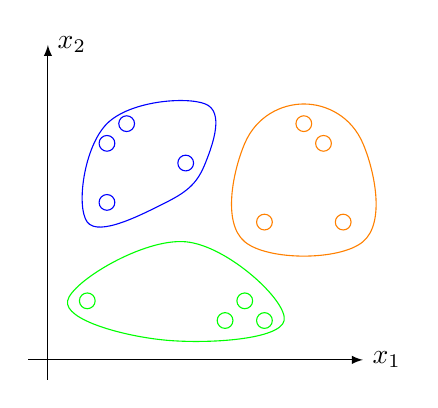
\begin{tikzpicture}[scale=.5]
\draw [-latex] (-.5,0) -- (8,0) node[right]{$x_1$};
\draw [-latex] (0,-.5) -- (0,8) node[right]{$x_2$};
\draw [blue] plot[smooth cycle, tension=.7] coordinates {(1.5,6) (1,3.5) (3,4) (4,5) (4,6.5)};
\draw [orange] plot[smooth cycle, tension=.7] coordinates {(6.5,6.5) (5,5.5) (5,3) (8,3) (8,5.5)};
\draw [green] plot[smooth cycle, tension=.7] coordinates {(0.5,1.5) (3.5,3) (6,1) (3,0.5)};
\draw [blue] (2,6) circle (0.2);
\draw [blue] (1.5,5.5) circle (0.2);
\draw [blue] (3.5,5) circle (0.2);
\draw [blue] (1.5,4) circle (0.2);
\draw [orange] (6.5,6) circle (0.2);
\draw [orange] (7,5.5) circle (0.2);
\draw [orange] (5.5,3.5) circle (0.2);
\draw [orange] (7.5,3.5) circle (0.2);
\draw [green] (1,1.5) circle (0.2);
\draw [green] (5.5,1) circle (0.2);
\draw [green] (4.5,1) circle (0.2);
\draw [green] (5,1.5) circle (0.2);
\end{tikzpicture}
\end{center}
\paragraph{Lernverfahren} 
\begin{itemize}
\item Versuche, die Lage der Referenzvektoren zu optimieren.
\item Nach Optimierung ist die Klassifikation von unbekannten Eingangsdaten möglich:\\
Das Klassenattribut des \emph{Best-Matching-Neurons} (-Referenzvektors) wird dem Eingangsdatum $\vec{x}$ zugeordnet (Zuweisung zum Referenzvektor, der am nächsten zum Eingangsvektor liegt).
\end{itemize}

\section{Optimierverfahren}
Für LVQ existieren \emph{viele} unterschiedliche Varianten.

\subsection{LVQ 1}
In jedem Adaptionsschritt  wird \emph{nur} das Best-Matching-Neuron (im Bezug zu der Menge der Beispiel- bzw.Trainingsdaten) angepasst.\\
Format der Trainingsdaten: $\vec{x}^{n}$ Label $k$\quad($k \in $ mögliche Klassen [in Beispiel $\tblue{1}, \torange{2}, \tgreen{3}$])

\subsubsection*{Lernalgorithmus}
\begin{enumerate}
\item Wähle ein $\vec{x}$ (aus Trainingsdaten).
\item Bestimme Best-Matching-Neuron $b$ nach Lernvorschrift:
$$\vec{w}_b=\underset{i=1\ldots P}{\operatorname{argmin}} \Vert \vec{x}-\vec{w}_i \Vert$$
Sowohl $\vec{x}$ als auch $\vec{w}_b$ verfügen über ihr jeweiliges Klassenlabel/-attribut.
\item Zwei Fälle abhängig davon, ob die Klassenattribute gleich sind oder nicht:
\begin{itemize}
\item Falls $\vec{x}$ und $\vec{w}_b$ gleiches Klassenattribut aufweisen:
$$\vec{w}_b(t+1) = \vec{w}_b(t)\tred{+}\eta(t)\left[ \vec{x}(t)-\vec{w}_b(t)\right]$$
$\To$ Verschiebung von $\vec{w}_b$ in Richtung $\vec{x}$.
\item Falls $\vec{x}$ und $\vec{w}_b$ verschiedene Klassenattribute aufweisen: 
$$\vec{w}_b(t+1) = \vec{w}_b(t)\tred{-}\eta(t)\left[ \vec{x}(t)-\vec{w}_b(t)\right]$$
$\To$ Verschiebung von $\vec{w}_b$ von $\vec{x}$ weg.
\end{itemize}
Zeitabhängige Lernrate $\eta(t)$ ist mit $\eta(t+1)=\eta(t)\cdot \alpha$ und $\eta(t=0)\approx 0.5$ definiert. Dabei liegt $0<\alpha\leq 1$, typische Größen sind $0.9,\; 0.99$ usw.\\
Durch die zeitabhängige Lernrate „friert“ die Verteilung irgendwann ein (und stellt somit den optimalen Zustand dar).\\
Wichtig: $t$ der Lernrate meint die gesamte Trainingsepoche (ein Mal mit allen Trainingsdaten trainiert).\\
Anmerkung: $\alpha=1$ wäre nur sinnvoll, wenn die Lernrate $\eta(t=0)$ sehr klein ist.
\end{enumerate}

\subsection{LVQ 2.1}
Im Unterschied zu LVQ 1:
\begin{itemize}
\item Nutzt sowohl Best-Matching-Neuron $b$ a-s auch Second-Best-Matching-Neuron $s$.
\item $\vec{x}$ muss in einem „Fenster“ bzw. zwischen $\vec{w}_b$ und $\vec{w}_s$ liegen:
\begin{center}
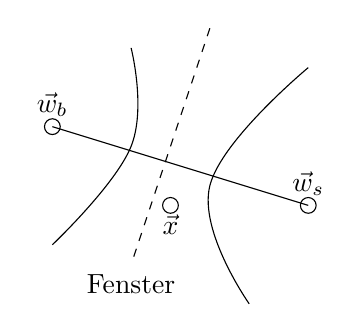
\begin{tikzpicture}[scale=.5]
\draw  plot[smooth, tension=.7] coordinates {(-2.5,4.5) (-2.5,2) (-4.5,-0.5)};
\draw  plot[smooth, tension=.7] coordinates {(2,4) (-0.5,1) (0.5,-2)};
\draw [dashed] (-0.5,5) -- (-2.5,-1) node[below]{Fenster};
\draw (-4.5,2.5) -- (2,0.5);
\draw  (-4.5,2.5) circle (0.2) node[above]{$\vec{w}_b$};
\draw  (2,0.5) circle (0.2) node[above]{$\vec{w}_s$};
\draw  (-1.5,0.5) circle (0.2) node[below]{$\vec{x}$};
\end{tikzpicture}
\end{center}
Falls $\vec{x}$ nicht in Fenster liegt, erfolgt \emph{keine} Adaption:
\begin{center}
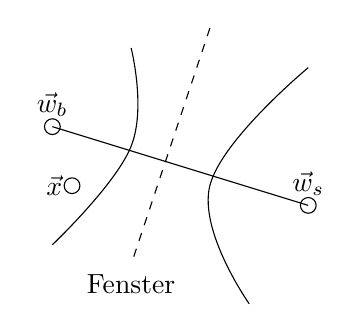
\begin{tikzpicture}[scale=.5]
\draw  plot[smooth, tension=.7] coordinates {(-2.5,4.5) (-2.5,2) (-4.5,-0.5)};
\draw  plot[smooth, tension=.7] coordinates {(2,4) (-0.5,1) (0.5,-2)};
\draw [dashed] (-0.5,5) -- (-2.5,-1) node[below]{Fenster};
\draw (-4.5,2.5) -- (2,0.5);
\draw  (-4.5,2.5) circle (0.2) node[above]{$\vec{w}_b$};
\draw  (2,0.5) circle (0.2) node[above]{$\vec{w}_s$};
\draw  (-4,1) circle (0.2) node[left]{$\vec{x}$};
\end{tikzpicture}
\end{center}
$\vec{w}_b$ und $\vec{w}_s$ müssen verschiedene Klassen repräsentieren!
\end{itemize}
Fenster: Wird aus Relationen zwischen den Abständen $d_b=\Vert \vec{x}-\vec{w}_b\Vert$ und $d_s=\Vert \vec{x}-\vec{w}_s\Vert$ berechnet. Mit $0.2\leq v \leq 0.3$ muss $\min\left(\frac{d_b}{d_s}, \frac{d_s}{d_b}\right)>\frac{1-v}{1+v}$ sein, damit $\vec{x}$ im Fenster liegt. 
\subsubsection*{Lernalgorithmus}
\begin{enumerate}
\item Wähle ein $\vec{x}$.
\item Bestimme Best- und Second-Best-Matching-Neuronen.
\item Prüfe, ob $\vec{x}$ im Fenster liegt. Falls $\vec{x}$ im Fenster, dann:
\begin{anumerate}
\item $\operatorname{Klasse}(\vec{w}_b) = \operatorname{Klasse} (\vec{x}(t))$
$$\vec{w}_b(t+1) = \vec{w}_b(t)+\eta(t)\cdot \left[ \vec{x}(t) - \vec{w}_b(t)\right]$$
$$\vec{w}_s(t+1) = \vec{w}_s(t)-\eta(t)\cdot \left[ \vec{x}(t) - \vec{w}_s(t)\right]$$
\item $\operatorname{Klasse}(\vec{w}_s) = \operatorname{Klasse} (\vec{x}(t))$
$$\vec{w}_b(t+1) = \vec{w}_b(t)-\eta(t)\cdot \left[ \vec{x}(t) - \vec{w}_b(t)\right]$$
$$\vec{w}_s(t+1) = \vec{w}_s(t)+\eta(t)\cdot \left[ \vec{x}(t) - \vec{w}_s(t)\right]$$
\end{anumerate}
\end{enumerate}
LVQ 2.1 adaptiert ausschließlich die Referenzvektoren, die entlang der Klassengrenzen liegen.\\
$\To$ Die Referenzvektoren, die „innerhalb“ der Klassengebiete liegen, bleiben unverändert. $\To$ Gegebenenfalls schlechte Generalisierung innerhalb der Klassengebiete.

\subsection{LVQ 3}
Arbeitet analog zu LVG 2.1 und lässt zusätzlich den Fall zu, dass $\operatorname{Klasse}(\vec{w}_b) = \operatorname{Klasse}(\vec{w}_s) = \operatorname{Klasse} (\vec{x}(t))$ gilt. Für diesen Fall werden $\vec{w}_b$ und $\vec{w}_s$ adaptiert mit:
$$\vec{w}_{b/s}(t+1)=\vec{w}_{b/s}(t)+\eta(t) \cdot \epsilon \cdot \left[\vec{x}(t)-\vec{w}_{b/s}(t)\right]$$
Dabei ist $\epsilon \approx 0.5$.\\
Damit kann auch innerhalb der Klassen adaptiert werden. Somit ist die Repräsentation der Statistik der Klassengebiete möglich.

\subsection{Optimized LVQ (OLVQ)}
Ziel ist, dass jedes Datum der Trainingsdaten den gleichen Einfluss auf die Lage des Referenzvektors hat. Dazu führt man für jeden Referenzvektor eine eigene Schrittweite, die dies sicherstellt.

\subsection{Handhabung der LVQ-Verfahren}
Die Performance/Güte eines LVQ-Netzwerks hängt von folgenden Faktoren ab:
\begin{anumerate}
\item Zahl der Referenzvektoren pro Klasse 
\item Initialisierung der Referenzvektoren
\item Verwendeten LVQ-Verfahren
\item Zeitlichem Verlauf der Lernrate
\item Einem geeigneten Abbruchkriterium
\end{anumerate}

Als „best praxis“ Vorgehen zeit sich oft:
\begin{enumerate}
\item Mit OLVQ-Training beginnen.
\item Mit LVQ 1 bzw. LVQ 3 nachtrainieren.
\end{enumerate}